\chapter[Metodologia]{Metodologia}

  A implementação do \textit{software} utilizará a metodologia ágil \textit{Extreme Programming (XP)} como ciclo de vida de desenvolvimento, dado o escopo, o nível de definição dos requisitos e o tamanho da equipe. O XP é um ciclo de vida de desenvolvimento voltado para projetos com equipes pequenas, sistemas orientados a objeto e com desenvolvimento incremental, segundo \citeonline{vinicius}. Sendo dividido em iterações que evoluem a aplicação de forma incremental. Primeiramente, é definido o escopo e as ferramentas a serem utilizadas. Então, há o desenvolvimento do protótipo e, por fim, o desenvolvimento da solução planejada.

  \section[Ferramentas Utilizadas]{Ferramentas Utilizadas}

    Antes do início da implementação da solução, foram escolhidas as ferramentas a serem utilizadas no projeto, de acordo com os requisitos levantados. Durante o desenvolvimento, essas serão as ferramentas utilizadas:

  \begin{enumerate}
    \item GitHub\footnotemark \footnotetext{\url{https://github.com/}}: plataforma para hospedagem de código-fonte que utiliza o Git como sistema de controle de versão. Será utilizado para o armazenamento do código da solução pelo seu caráter aberto e gratuito;
    \item C++\footnotemark \footnotetext{\url{http://www.cplusplus.com/}}, linguagem de programação compilada multiparadigma. Será utilizada como linguagem de implementação principal pelo suporte à programação orientada a objetos e domínio dela pela equipe;
    \item Lilypond\footnotemark \footnotetext{\url{http://lilypond.org/}}, formato de escrita musical baseado em TeX. Será utilizado para representação da melodia por ter um formato padronizado e menos verboso se comparado a outras opções como o MusicXML. Além disso, seu pacote para Linux conta com métodos como midi2ly e musicxml2ly que permite converter músicas de formatos populares para o formato .ly padrão do Lilypond;
    \item MuseScore\footnotemark \footnotetext{\url{https://musescore.com/}}, editor de partituras. Será utilizado para criação e edição de partitura pelo fato da equipe ter domínio sobre a ferramenta e ser compatível com Linux e Windows, ao contrário de alternativas similares como o Encore;
  \end{enumerate}

  \section[Ciclo de Vida de Desenvolvimento]{Ciclo de Vida de Desenvolvimento}

    O ciclo de vida de desenvolvimento contará com três fases bem definidas. Primeiramente, serão levantados os requisitos. Então, serão escolhidas as ferramentas a serem utilizadas. Após isso, será desenvolvido um protótipo focado em contrapontos de primeira espécie. Os resultados do protótipo guiarão o desenvolvimento posterior, que será focado na composição algorítmica de contrapontos palestrinianos de até quinta espécie.

  \subsection[Requisitos]{Requisitos}

    Os requisitos foram desenvolvidos na primeira parte do trabalho. O escopo inicial era de um \textit{software} capaz de ler uma melodia monofônica e gerar contrapontos palestrinianos de até quinta espécie para ela, retornando o este no mesmo formato lido, com o formato escolhido sendo o Lilypond. Veja um fluxograma simplificado da aplicação na Figura \ref{fluxograma}.

    \begin{figure}[htb]
      \centering
      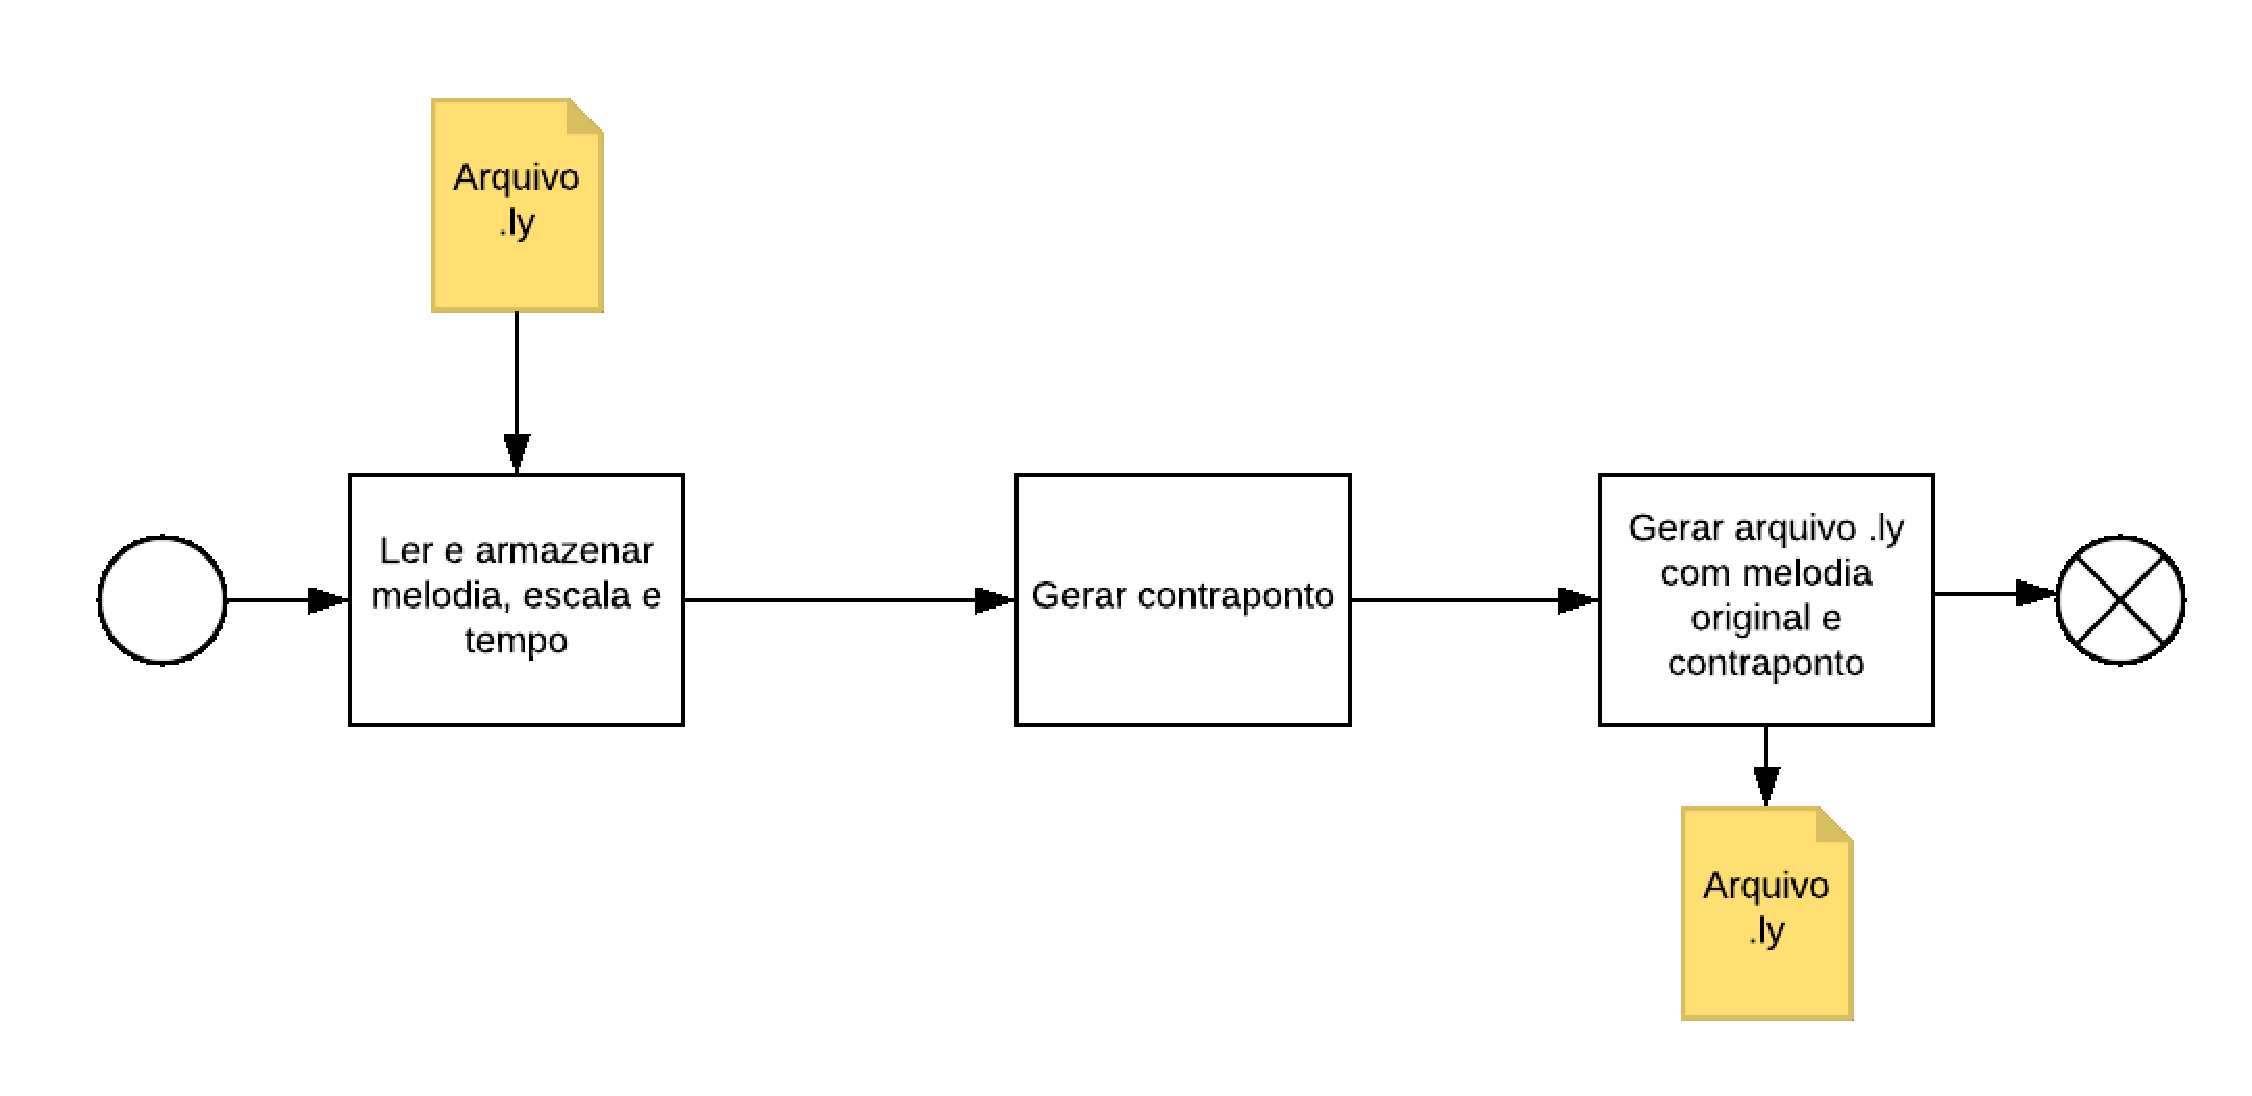
\includegraphics[scale=0.45]{figuras/fluxograma.eps}
      \caption{Fluxograma simplificado da aplicação}
      \label{fluxograma}
    \end{figure}


    Após o estudo da teoria musical necessária para a construção de contrapontos,foram definidos os seguintes módulos a serem desenvolvidos:

    \begin{enumerate}
      \item Módulo de notas musicais;
      \item Módulo de intervalos;
      \item Módulo de escalas;
      \item Módulo de contrapontos de primeira espécie;
      \item Módulo de contrapontos de segunda espécie;
      \item Módulo de contrapontos de terceira espécie;
      \item Módulo de contrapontos de quarta espécie;
      \item Módulo de contrapontos de quinta espécie;
      \item Módulo de construção do MIDI.
    \end{enumerate}

    \subsubsection[Módulo de Notas Musicais]{Módulo de Notas Musicais}

      Este módulo é responsável pela leitura e armazenamento das notas de uma melodia. Ele conta com as seguintes capacidades: armazenamento do atributos de uma nota, \textit{parser} de uma nota em formato Lilypond e armazenamento de uma melodia completa. O armazenamento de uma nota inclui tais atributos: a figura musical que representa a duração, o tempo absoluto da nota, os acidentes aplicados a ela, a oitava em que ela está inserida, seu número MIDI e seu número em relação a notas sem contar acidentes. Além disso, essa parte deve ser capaz de devolver notas enarmônicas a uma nota -- notas com nomenclatura diferente, mas som e número de semitons (em relação a uma nota qualquer) iguais, como C\sh{}  e D\fl.

      O \textit{parser} de uma nota deve ser feito a partir de um arquivo Lilypond e armazenado na estrutura responsável pelo armazenamento de notas já citada. Além disso, ele deve ser capaz de retornar uma nota armazenada no mesmo formato lido.

      O armazenamento da melodia completa deve ser capaz de armazenar as notas de uma melodia preservando sua ordem, além de armazenar o tempo dos compassos e a escala da música.

    \subsubsection[Módulo de Intervalos]{Módulo de Intervalos}

      O módulo de intervalos deve ser capaz de armazenar intervalos, gerá-los a partir de duas notas ou de uma \textit{string} e ser capaz de retornar a outra nota dados uma nota e um intervalo, por exemplo, retornar G\sh5 ao receber C5 e um intervalo de quinta aumentada.

      O armazenamento de intervalos deve possuir os seguintes atributos: classificaçõs quantitativa e qualitativa, número de semitons e se o intervalo é ascendente ou não (considerando a nota recebida como a primeira).

      O retorno da nota dado uma nota e um intervalo deve ser capaz de retornar a segunda nota para qualquer intervalo definido, de forma que a distância entre as duas notas seja compatível com a classificação quantitativa e qualitativa do intervalo. Ele também deve ser capaz de indicar se é impossível gerar tal nota e retornar uma nota em uma dada escala previamente definida, quando necessário.

    \subsubsection[Módulo de Escalas]{Módulo de Escalas}

      O módulo de escalas deve ser capaz de armazenar uma escala e responder se uma nota faz ou não parte dela. O armazenamento da escala deve ser capaz de armazenar quais notas estão presentes nela a partir da primeira nota e do modo (maior ou menor) ou da primeira nota e de um conjunto de intervalos.

      O objeto de uma escala deve ser capaz de receber um objeto de nota e dizer se aquela nota está ou não presente, baseada em seu número de MIDI e sua representação, por exemplo, a nota B está presente na escala de Dó Maior, mas não a nota C\fl{}, embora elas sejam enarmônicas.

    \subsubsection[Módulos de Contraponto]{Módulo de Contraponto}

      Cada módulo deve ser capaz de gerar um contraponto palestriniano de acordo com as regras definidas pela espécie do contraponto. Eles devem receber uma melodia monofônica e gerar um contraponto daquela espécie de acordo com os parâmetros fornecidos em relação a número de movimentos reversos, consonâncias condicionais paralelas e outros parâmetros relacionados a regras que não sejam exatas. Como exemplo, tem-se a regra que se evita, mas não se proíbe movimentos paralelos, cabendo ao usuário definir o número de movimentos paralelos aceitáveis. Com tais parâmetros, o módulo deve ser capaz de gerar um contraponto aleatório para cada iteração do algoritmo.

    \subsubsection[Módulo de Construção do MIDI]{Módulo de Construção do MIDI}

      O módulo de construção do MIDI é um módulo que deve automatizar a construção de um MIDI tendo como base o arquivo Lilypond original e o contraponto gerado. Com esses dois, esse módulo deve inserir o contraponto em uma cópia do arquivo original e gerar o MIDI utilizando o pacote do Lilypond para Linux.

  \subsection[Protótipo]{Protótipo}

    Assim como os requisitos, o protótipo também foi desenvolvido na primeira parte do trabalho. O protótipo possui a finalidade de testar o conceito da solução por meio um MVP (produto mínimo viável ou \textit{minimum viable product}). O protótipo proposto possuía as seguintes funcionalidades:

    \begin{enumerate}
      \item Módulo de notas musicais, incluindo leitura de arquivo Lilypond simplificado e armazenamentos de notas de uma melodia;
      \item Módulo de intervalos, incluindo a construção de intervalos a partir de notas ou \textit{strings} padronizadas e retorno de nota ao se receber nota e intervalo;
      \item Módulo de escalas, incluindo construção de escalas a partir do modo ou de um conjunto de intervalos;
      \item Módulo de contrapontos de primeira espécie implementado utilizando busca completa;
      \item Módulo de contrapontos de primeira espécie implementado utilizando programação;
      \item Módulo de contrapontos de segunda espécie, com leitura de tempo de compasso.
    \end{enumerate}

    O protótipo contém os módulos de notação, intervalos e escalas pois são considerados módulos básicos para a construção de contrapontos.

    O módulo de contrapontos de primeira espécie com algoritmo de busca completa pretende testar se a geração de contrapontos de forma \textit{naive} (a implementação mais simples possível) é correta e computacionalmente viável.

    O módulo de contrapontos de segunda espécie com algoritmo de DP pretende testar se a programação dinâmica efetivamente diminui o tempo de execução do algoritmo e se essa diminuição é relevante o suficiente para justificar o uso desse paradigma.

    O módulo de contrapontos de segunda espécie busca validar a corretude do módulo de primeira espécie uma vez que tenha sido escalado. Dentre as novas dificuldades, há o fato de que há duas notas no contraponto para cada do \textit{cantus firmus}, a posição da nota no compasso possui papel decisivo no algoritmo, invalidando a estratégia de avaliar os intervalos nota a nota e adicionando um estado à DP.

  \subsection[Desenvolvimento]{Desenvolvimento}

    Após a definição dos requisitos e a construção do protótipo, o sistema terá o restante de suas funcionalidades implementadas e testadas. As atividades previstas para a fase de desenvolvimento são:

    \begin{enumerate}
      \item Testes dos módulos de notação, intervalos e escalas;
      \item Testes dos módulos de contraponto de primeira e segunda espécie;
      \item Otimização do \textit{parser};
      \item Implementação e testes do módulo de contrapontos de terceira espécie;
      \item Implementação e testes do módulo de contrapontos de quarta espécie;
      \item Implementação e testes do módulo de contrapontos de quinta espécie;
      \item Implementação e testes do módulo de construção de MIDI.
    \end{enumerate}

    A segunda parte do trabalho, que engloba o desenvolvimento, começará com testes das funcionalidades implementadas no protótipo. O objetivo é garantir que a solução do protótipo é adequada e completa antes de começar a implementação definitiva, refatorando o código e removendo \textit{bugs} identificados.

    Após isso, há a otimização do \textit{parser}. O \textit{parser} atual lê apenas um arquivo Lilypond modificado para conter apenas o tempo, a escala e as notas. Pretende-se criar um \textit{parser} que, ainda que simples, seja capaz de ler arquivos Lilypond padrão.

    Seguindo a otimização do \textit{parser}, haverá a implementação e teste dos contrapontos de terceira, quarta e quinta espécie. Baseado no código já implementado dos contrapontos de primeira e segunda espécie, eles serão desenvolvidos sequencialmente, já que as novas regras de uma espécie somam-se às regras da anterior.

    Por fim, haverá a implementação e teste de um módulo de construção de MIDI com as especificações definidas na subseção acerca dos requisitos.

  \section[Atividades e Cronograma]{Atividades e Cronograma}

  O desenvolvimento do sistema terá as seguintes atividades:

  \begin{enumerate}
    \item \label{t1} Definição dos requisitos do sistema;
    \item \label{t2} Estudo sobre teoria musical, incluindo notação musical, intervalos, escalas e contrapontos;
    \item \label{t3} Implementação do protótipo de parser de um arquivo lilypond;
    \item \label{t4} Implementação do módulo de notas musicais;
    \item \label{t5} Implementação do módulo de intervalos;
    \item \label{t6} Implementação do módulo de escalas;
    \item \label{t7} Implementação do protótipo do módulo de contrapontos;
    \item \label{t8} Implementação do módulo de contrapontos de primeira espécie utilizando busca completa;
    \item \label{t9} Implementação do módulo de contrapontos de primeira espécie utilizando programação dinâmica;
    \item \label{t10} Escrita do TCC1;
    \item \label{t11} Implementação do módulo de contrapontos de segunda espécie;
    \item \label{t12} Testes do parser;
    \item \label{t13} Testes do módulo de notas musicais;
    \item \label{t14} Testes do módulo de intervalos;
    \item \label{t15} Testes do módulo de escalas;
    \item \label{t16} Testes dos módulos de contrapontos de primeira e segunda espécie;
    \item \label{t17} Otimização do parser;
    \item \label{t18} Implementação e testes do módulo de contrapontos de terceira espécie;
    \item \label{t19} Implementação e testes do módulo de contrapontos de quarta espécie;
    \item \label{t20} Implementação e testes do módulo de contrapontos de quinta espécie;
    \item \label{t21} Implementação e testes do módulo de construção de MIDI;
    \item \label{t22} Escrita do TCC2.
  \end{enumerate}

  O cronograma do trabalho está apresentado na Tabela \ref{tab:cronograma}.

  \definecolor{midgray}{gray}{.5}
  \begin{table}[!htbp]
    \centering
    \caption{Cronograma do Trabalho}
    \label{tab:cronograma}
      \begin{tabular}{|c|c|c|c|c|c|c|c|c|c|c|}
      \hline
      &\multicolumn{10}{c|}{2018}\\
      \hline
      &MAR&ABR&MAI&JUN&JUL&AGO&SET&OUT&NOV&DEZ\\
      \hline
      \ref{t1}&\cellcolor{green}&&&&&&&&&\\
      \hline
      \ref{t2}&\cellcolor{green}&\cellcolor{green}&&&&&&&&\\
      \hline
      \ref{t3}&\cellcolor{green}&&&&&&&&&\\
      \hline
      \ref{t4}&\cellcolor{green}&&&&&&&&&\\
      \hline
      \ref{t5}&&\cellcolor{green}&&&&&&&&\\
      \hline
      \ref{t6}&&&\cellcolor{green}&&&&&&&\\
      \hline
      \ref{t7}&&\cellcolor{green}&\cellcolor{green}&&&&&&&\\
      \hline
      \ref{t8}&&\cellcolor{green}&&&&&&&&\\
      \hline
      \ref{t9}&&\cellcolor{green}&\cellcolor{green}&&&&&&&\\
      \hline
      \ref{t10}&&\cellcolor{green}&\cellcolor{green}&\cellcolor{green}&&&&&&\\
      \hline
      \ref{t11}&&&&\cellcolor{yellow}&\cellcolor{yellow}&&&&&\\
      \hline
      \ref{t12}&&&&&\cellcolor{red}&\cellcolor{red}&&&&\\
      \hline
      \ref{t13}&&&&&\cellcolor{red}&\cellcolor{red}&&&&\\
      \hline
      \ref{t14}&&&&&\cellcolor{red}&\cellcolor{red}&&&&\\
      \hline
      \ref{t15}&&&&&\cellcolor{red}&\cellcolor{red}&&&&\\
      \hline
      \ref{t16}&&&&&\cellcolor{red}&\cellcolor{red}&&&&\\
      \hline
      \ref{t17}&&&&&&\cellcolor{red}&&&&\\
      \hline
      \ref{t18}&&&&&&\cellcolor{red}&\cellcolor{red}&&&\\
      \hline
      \ref{t19}&&&&&&&\cellcolor{red}&\cellcolor{red}&&\\
      \hline
      \ref{t20}&&&&&&&&\cellcolor{red}&\cellcolor{red}&\\
      \hline
      \ref{t21}&&&&&&&&&\cellcolor{red}&\cellcolor{red}\\
      \hline
      \ref{t22}&&&&&&&&\cellcolor{red}&\cellcolor{red}&\cellcolor{red}\\
      \hline
      \multicolumn{11}{|c|}{Legendas}\\ \hline
      \multicolumn{10}{|l|}{Tarefas não realizadas} &\cellcolor{red}\\
      \hline
      \multicolumn{10}{|l|}{Tarefas em andamento} &\cellcolor{yellow}\\
      \hline
      \multicolumn{10}{|l|}{Tarefas realizadas}&\cellcolor{green}\\
      \hline
      \end{tabular}
  \end{table}
